\documentclass[12pt,a4psprt]{article}
\usepackage[spanish]{babel}
\usepackage[utf8]{inputenc}
\usepackage{eurosym}
\usepackage[pdftex]{graphicx}     
\usepackage{listings}

\lstset{literate=
  {á}{{\'a}}1 {é}{{\'e}}1 {í}{{\'i}}1 {ó}{{\'o}}1 {ú}{{\'u}}1
  {Á}{{\'A}}1 {É}{{\'E}}1 {Í}{{\'I}}1 {Ó}{{\'O}}1 {Ú}{{\'U}}1
  {à}{{\`a}}1 {è}{{\`e}}1 {ì}{{\`i}}1 {ò}{{\`o}}1 {ù}{{\`u}}1
  {À}{{\`A}}1 {È}{{\'E}}1 {Ì}{{\`I}}1 {Ò}{{\`O}}1 {Ù}{{\`U}}1
  {ä}{{\"a}}1 {ë}{{\"e}}1 {ï}{{\"i}}1 {ö}{{\"o}}1 {ü}{{\"u}}1
  {Ä}{{\"A}}1 {Ë}{{\"E}}1 {Ï}{{\"I}}1 {Ö}{{\"O}}1 {Ü}{{\"U}}1
  {â}{{\^a}}1 {ê}{{\^e}}1 {î}{{\^i}}1 {ô}{{\^o}}1 {û}{{\^u}}1
  {Â}{{\^A}}1 {Ê}{{\^E}}1 {Î}{{\^I}}1 {Ô}{{\^O}}1 {Û}{{\^U}}1
  {œ}{{\oe}}1 {Œ}{{\OE}}1 {æ}{{\ae}}1 {Æ}{{\AE}}1 {ß}{{\ss}}1
  {ű}{{\H{u}}}1 {Ű}{{\H{U}}}1 {ő}{{\H{o}}}1 {Ő}{{\H{O}}}1
  {ç}{{\c c}}1 {Ç}{{\c C}}1 {ø}{{\o}}1 {å}{{\r a}}1 {Å}{{\r A}}1
  {€}{{\EUR}}1 {£}{{\pounds}}1 {ñ}{{\~n}}1 {Ñ}{{\~n}}1
}

\pagestyle{plain}
\title{\fbox{\fbox{\bf Práctica 1: Eficiencia}}}
\author{Antonio Jesús Heredia Castillo\\ 2ºA \\ ETS de Ingenierías Informática y de Telecomunicación }
\date{\today}
\begin{document}
%portada
\maketitle{}
	
\begin{abstract}
En esta practica obtendremos datos sobre el tiempo de ejecucion de distintos algoritmos y como afecta la compilacion al tiempo de ejecución.
\end{abstract}



%indice
\pagebreak
\tableofcontents
\pagebreak
\section{Ejercicio 1: Dependencia del entorno}
\subsection{Sistema usado}
Acontinuacion se adjunta una tabla con el hardware usado: \\
\begin{center}
\begin{tabular}{|l||r|p{2cm}}
\hline
\multicolumn{2}{|c|}{Hardware} \\
\hline
CPU & Intel(R) Core(TM) i5-6600 \\
\hline
Velocidad de reloj & 3.30GHz \\
\hline
Arquitectura & 64bits \\
\hline
Memoria RAM & 16GB \\
\hline
Tipo de maquina & x86\_64 \\
\hline

\end{tabular}
\end{center}

El sistema operativo usado a sido : \textbf{Linux Mint 18.1 Serena}.
\subsection{Codigo}
El codigo del programa principal es el siguiente:
\begin{lstlisting}[language=C++]
#include <iostream>
#include <ctime>    // Recursos para medir tiempos
#include <cstdlib>  // Para generacion de numeros pseudoaleatorios
using namespace std;

void forma_usar(void){
	cerr << "Numero de parametro incorrecto" << endl;
	cerr << "Forma correcta de ejecutar: " << endl;
	cerr << "ejercicio7_1 tamaño valor_maximo" << endl;
	exit(1);
}

//Codigo copiado del PDF de practicas
void ordenar(int *v, int n) {
	bool cambio=true;
	for (int i=0; i<n-1 && cambio; i++) {
		cambio=false;
		for (int j=0; j<n-i-1; j++)
			if (v[j]>v[j+1]) {
				cambio=true;
				int aux = v[j];
				v[j] = v[j+1];
				v[j+1] = aux;
			}
	}
}

int main(int argc, char * argv[])
{
	if (argc!=3)
		forma_usar();
	int tam=atoi(argv[1]);     // Tamaño del vector
	int max=atoi(argv[2]);    // Valor maximo
	
	if (tam<=0 || max<=0)
    	forma_usar();
  
	// Generacion del vector aleatorio
	int *v=new int[tam];       // Reserva de memoria.
	// Inicializacion del generador de numeros pseudoaleatorios
	srand(time(0));            
	for (int i=0; i<tam; i++)  // Recorrer vector
		v[i] = rand() % max;    // Generar aleatorio [0,max[

	clock_t tini;    // Anotamos el tiempo de inicio
	tini=clock();

	ordenar(v,tam); // de esta forma forzamos el peor caso
  
	clock_t tfin;    // Anotamos el tiempo de finalizaciun
	tfin=clock();

	// Mostramos resultados
	cout << tam << "\t" << (tfin-tini)/(double)CLOCKS_PER_SEC 
	<< endl;
  
  delete [] v;     // Liberamos memoria dinamica
}

\end{lstlisting}

El programa ha sido compilado con un fichero makefile que contenia la orden:
\begin{verbatim}
$g++ -O3 -o ejercicio_7_1 ejercicio_7_1.cpp
\end{verbatim}
Para obtener los datos he usado un script parecido al del PDF de la practica pero adaptado para la shell de bash. Los datos obtenidos seran los usados para obtener los puntos de la grafica con la que veremos la eficiencia.
\begin{lstlisting}[language=bash]
#!/bin/bash
#Nombre del fichero: ejecucion_ejercicio_7_1.sh
#Funcion: El script ejecuta el programa de ordenacion para obtener datos de eficiencia
INICIO=100
FIN=20000
INCREMENTO=100
EJECUTABLE=./bin/ejercicio_7_1
SALIDA=tiempoOrdenacion.dat

i=$INICIO
echo > $SALIDA
while [ $i -lt $FIN ];do
  echo Ejecucion tam = $i
  $EJECUTABLE $i 10000 >> $SALIDA
  let i+=$INCREMENTO
done

\end{lstlisting}

Una vez ejecutado el script obtendremos un fichero llamado \textbf{tiempoOrdenacion.dat} en el cual se encuentra en cada fila, en la primera columna el tamaño de la muestra y en la segunda el tiempo en segundos que ha tardado en realizar la ordenacion.
\pagebreak
\\
Apartir de los datos obtenidos  podemos realizar una grafica para ver si la eficiencia teoria que en este caso seria O($n^{2}$) corresponde con la eficiencia empirica. Donde la funcion tendria la siguiente forma: \textbf{$f(x)=a*x^{2}+b $}
\begin{figure}[h]
\begin{center}
	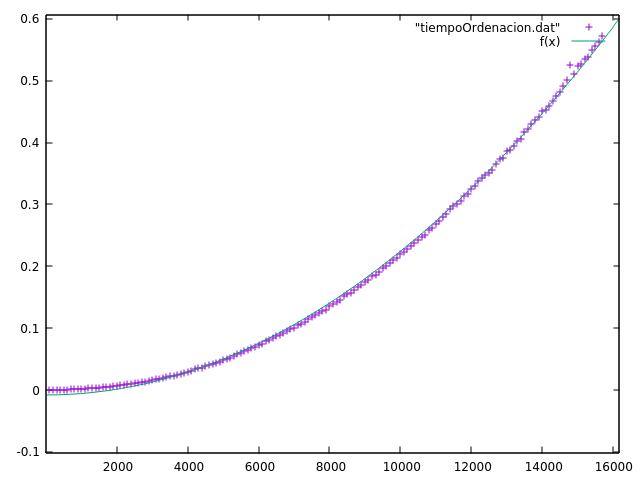
\includegraphics[scale=1]{image/grafica_7_1.png}
\end{center}
\caption{Grafica ejercicio 7.1}

\end{figure}
\\
Gracias a gnuplot podemos obtener el ajuste para a y b en f(x) para los datos obtenidos.
He obtenido que $a=-2.32*10^{-9}$ y $b=-0.0079$
\section{Ejercicio 2: Multiplicación matricial}
\subsection{Sistema usado}
Acontinuacion se adjunta una tabla con el hardware usado: \\
\begin{center}
\begin{tabular}{|l||r|p{2cm}}
\hline
\multicolumn{2}{|c|}{Hardware} \\
\hline
CPU & Intel(R) Core(TM) i5-6600 \\
\hline
Velocidad de reloj & 3.30GHz \\
\hline
Arquitectura & 64bits \\
\hline
Memoria RAM & 16GB \\
\hline
Tipo de maquina & x86\_64 \\
\hline

\end{tabular}
\end{center}

El sistema operativo usado a sido : \textbf{Linux Mint 18.1 Serena}.
\subsection{Codigo}
El codigo del programa principal es el siguiente:
\begin{lstlisting}[language=C++]
#include <iostream>
#include <ctime>    // Recursos para medir tiempos
#include <cstdlib>  // Para generación de números pseudoaleatorios

using namespace std;

void forma_usar(void){
	cerr << "Numero de parametro incorrecto" << endl;
	cerr << "Forma correcta de ejecutar: " << endl;
	cerr << "ejercicio7_2 tamaño " << endl;
	exit(1);
}

void multiplicar(int **m1, int **m2, int **m3, int tam) {
	
	for(int c = 0; c < tam; c++)
		for(int f = 0; f < tam; f++){
			int suma = 0;
			
			for(int x = 0; x < tam; x++)
				suma += m1[f][x]*m2[c][x];

			m1[f][c] = suma;
		}
			
	
}

int main(int argc, char * argv[])
{
  
	if (argc!=3)
		forma_usar();
	int tam=atoi(argv[1]);     // Tamaño de la matriz
	int max=atoi(argv[2]);

	if (tam<=0)
    	forma_usar();


	int **matriz1;
	int **matriz2;
	int **matriz3;

  	matriz1 = new int * [tam];
	matriz2 = new int * [tam];
	matriz3 = new int * [tam];

	for(int f = 0; f < tam; f++){
		matriz1[f] = new int  [tam];
		matriz2[f] = new int  [tam];
		matriz3[f] = new int  [tam];
	
	}
 	// Inicialización del generador de números pseudoaleatorios
	srand(time(0));           
	for(int f = 0; f < tam; f++)
		for(int c = 0 ; c < tam; c++){
			matriz1[f][c] = rand() % max; 
			matriz2[f][c] = rand() % max; 
		}
	

	clock_t tini;    // Anotamos el tiempo de inicio
	tini=clock();

	multiplicar(matriz1, matriz2, matriz3, tam);
	
	clock_t tfin;    // Anotamos el tiempo de finalización
	tfin=clock();

	// Mostramos resultados
	cout << tam << "\t" 
	<< (tfin-tini)/(double)CLOCKS_PER_SEC << endl;
  
	for(int f = 0; f < tam; f++){
		delete matriz1[f];
		delete matriz2[f];
		delete matriz3[f];
	}     // Liberamos memoria dinámica
	
	delete matriz1;
	delete matriz2;
	delete matriz3;
	
}

\end{lstlisting}

El programa ha sido compilado con un fichero makefile que contenia la orden:
\begin{verbatim}
$g++ -O3 -o ejercicio_7_2 ejercicio_7_2.cpp
\end{verbatim}
\pagebreak
Para obtener los datos he usado un script. Los datos obtenidos seran los usados para obtener los puntos de la grafica con la que veremos la eficiencia.
\begin{lstlisting}[language=bash]
#!/bin/bash
#Nombre del fichero: ejecucion_ejercicio_7_1.sh
#Funcion: El script ejecuta el programa de ordenacion 
#	para obtener datos de eficiencia
INICIO=100
FIN=3000
INCREMENTO=100
EJECUTABLE=./bin/ejercicio_7_2
SALIDA=tiempoMultiplicacion.dat

make
i=$INICIO
echo > $SALIDA
while [ $i -lt $FIN ];do
  echo Ejecución tam = $i
  $EJECUTABLE $i $FIN >> $SALIDA
  let i+=$INCREMENTO
done

\end{lstlisting}
\pagebreak
En este caso la eficiencia teorica seria O($n^{3}$) y por lo tanto no se puede ajustar correctamente con una funcion del estilo: \textbf{$f(x)=a*x^{2}+b $}.
\begin{figure}[h]
\begin{center}
	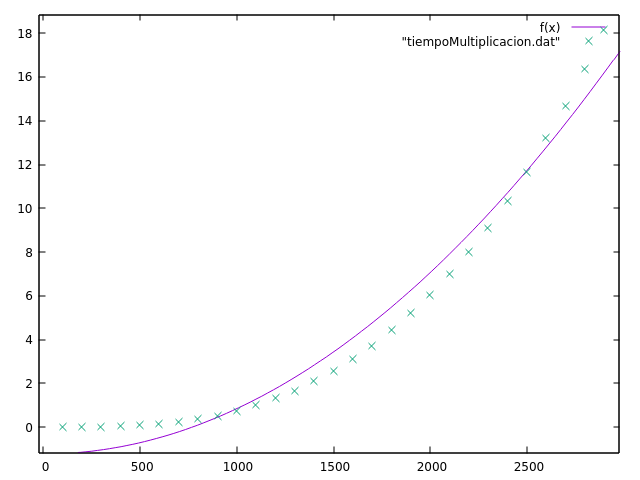
\includegraphics[scale=1]{image/grafica_7_2_cuadratica.png}
\end{center}
\caption{Grafica ejercicio 7.2 cuadratica}
\end{figure}
\\Como podemos obserbar la linea de f(x) en este caso no se ajusta de forma exacta a la nube de puntos de los datos que hemos obtenido.\\
\pagebreak
\\En cambio con \textbf{$f(x)=a*x^{3}+b $} si que se ajustaria bien la eficiencia teoriaca con la eficiencia empirica.\\.

\begin{figure}[h]
\begin{center}
	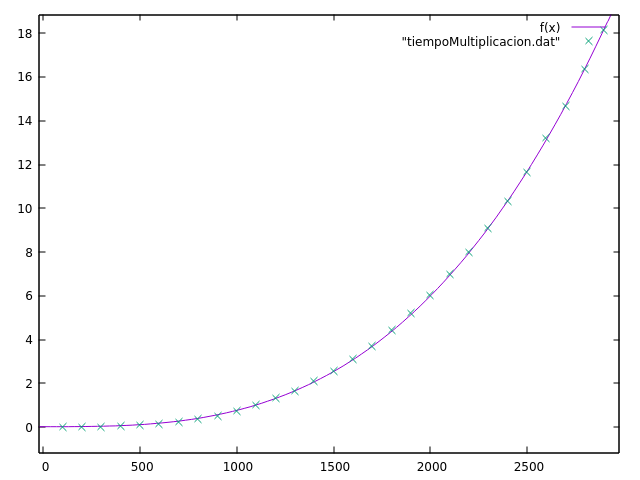
\includegraphics[scale=1]{image/grafica_7_2_cubica.png}
\end{center}
\caption{Grafica ejercicio 7.2 cubica}

\end{figure}
Gracias a gnuplot podemos obtener el ajuste para a y b en f(x) para los datos obtenidos.
He obtenido que $a=$ y $b=$

\end{document}